\documentclass[a4paper,12pt]{article}
\usepackage[margin=0.5in]{geometry}
\usepackage{amsmath}
\usepackage{accents}
\newcommand*{\dt}[1]{%
  \accentset{\mbox{\large\bfseries .}}{#1}}
\newcommand*{\ddt}[1]{%
  \accentset{\mbox{\large\bfseries .\hspace{-0.25ex}.}}{#1}}
\usepackage{graphicx}
\graphicspath{ {images/} } 
\usepackage{calrsfs}
\DeclareMathAlphabet{\pazocal}{OMS}{zplm}{m}{n}
\newcommand{\La}{\mathcal{L}}
\newcommand{\Lb}{\pazocal{L}}
\begin{document}

the model we use is called constant turn rate and velocity magnitude model (CTRV)
\begin{figure}[h!]
  \caption{state variables and their meaning}
  \centering
    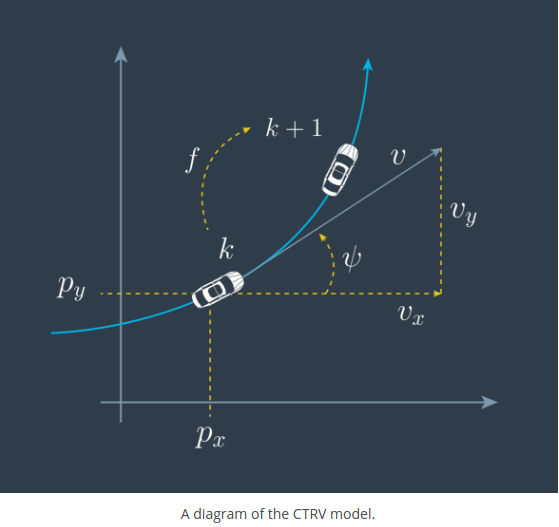
\includegraphics[scale=.5]{1.png}
\end{figure}

  \begin{align}
    x &= \begin{bmatrix}
         p_{x} \\
         p_{y} \\ 
         v \\
         \psi \\
         \dot{\psi} \\
         \end{bmatrix}
  \end{align}
  
  
  \begin{align}
    \dot{x} &= \begin{bmatrix}
         v\cos(\psi) \\
         v\sin(\psi) \\
         0 \\
         \dt{\psi} \\
         0 \\
         \end{bmatrix}
  \end{align}

  \begin{align}  
  x_{k+1}=x_k + \int_{t_k}^{t_{k+1}} 
  		 \begin{bmatrix}
         v\cos(\psi) \\
         v\sin(\psi) \\
         0 \\
         \dt{\psi} \\
         0 \\
         \end{bmatrix} dt 
  \end{align}
  
  
  
     \begin{align}  
  x_{k+1}=x_k +  
  		 \begin{bmatrix}
         v_k\int_{t_k}^{t_{k+1}}\cos(\psi_k+\dt{\psi_k}(t-t_k) dt \\
         v_k\int_{t_k}^{t_{k+1}}\sin(\psi_k+\dt{\psi_k}(t-t_k) dt\\
         0 \\
         \dt{\psi_k}\Delta t \\
         0 \\
         \end{bmatrix} 
  \end{align} 
  
   \begin{align}  
  x_{k+1}=x_k + 
  		 \begin{bmatrix}
         \frac{v_k}{\dt{\psi_k}}\left(\sin(\psi_k+\dt{\psi_k} \Delta t) -\sin(\psi_k) \right)\\
         \frac{v_k}{\dt{\psi_k}}\left(-\cos(\psi_k+\dt{\psi_k} \Delta t) +\cos(\psi_k) \right)\\
         0 \\
         \dt{\psi_k}\Delta t \\
         0 \\
         \end{bmatrix} 
  \end{align} 
  
when $\dt{\psi_k}=0$, the 2 top expressions in the integral are no longer functions of time, and can be pulled out of the integration, then the relationship becomes :

   \begin{align}  
  x_{k+1}=x_k + 
  		 \begin{bmatrix}
         v_k\cos(\psi_k)\Delta t\\
         v_k\sin(\psi_k)\Delta t\\
         0 \\
         0 \\
         0 \\
         \end{bmatrix} 
  \end{align} 

\begin{figure}[h!]
  \caption{state transition using differential equations}
  \centering
    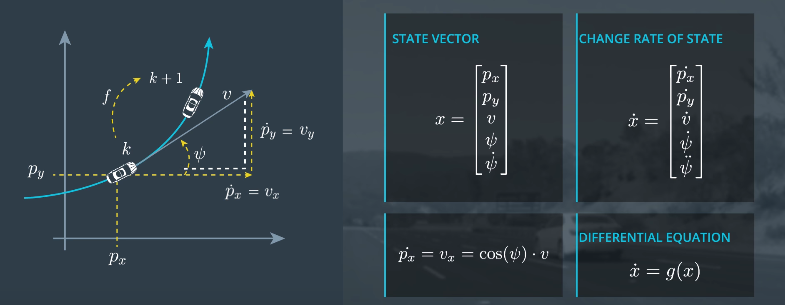
\includegraphics[scale=.5]{2.png}
    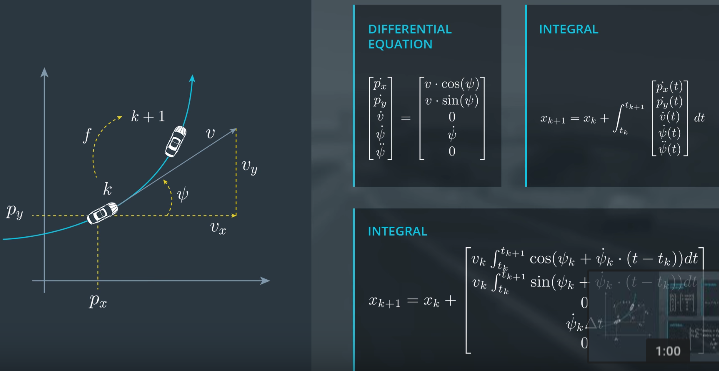
\includegraphics[scale=.5]{3.png}
\end{figure}

process noise is comprised of longitudenal and angular acceleration. This represents driver speeding up and slowing down during straight segments of the road or during turns. Constant turn rate and velocity magnitude model does not consider acceleration and they are added to the model as noise. in the UKF community this is called process noise ! however in EKF process noise was the random variable with same dimension as the state with mean $0$ and covariance $Q$.

   \begin{align}  
  \nu_{k}=
  		 \begin{bmatrix}
         \nu_{a,k}\\
         \nu_{\ddt{\psi},k}\\
         \end{bmatrix} 
         \sim N(
         \begin{bmatrix}
          0  \\
          0  \\
		 \end{bmatrix},     
         \begin{bmatrix}
    \sigma^2_a       & 0  \\
    0       & \sigma^{2}_{\ddt{\psi}}  \\
		\end{bmatrix} )
  \end{align} 
Here in UKF realm we define Q as 
   \begin{align}  
  Q =
    \begin{bmatrix}
    \sigma^2_a & 0  \\
    0  & \sigma^{2}_{\ddt{\psi}}  \\
	\end{bmatrix} 
  \end{align} 
assuming that you have a realization of the above random variables at time $k$ denoted by $\nu_{a,k}$ and $\nu_{\ddt{\psi},k}$, also assume that these values do not change from $k$ to $k+1$. The following is the impact of the realizations on the state. 

   \begin{align}  
  x_{k+1}=x_k + 
  		 \begin{bmatrix}
         \frac{v_k}{\dt{\psi_k}}\left(\sin(\psi_k+\dt{\psi_k} \Delta t) -\sin(\psi_k) \right)\\
         \frac{v_k}{\dt{\psi_k}}\left(-\cos(\psi_k+\dt{\psi_k} \Delta t) +\cos(\psi_k) \right)\\
         0 \\
         \dt{\psi_k}\Delta t \\
         0 \\
         \end{bmatrix} 
+
  		 \begin{bmatrix}
         \frac{1}{2}\Delta t^2\cos(\psi_k)\nu_{a,k}\\
         \frac{1}{2}\Delta t^2\sin(\psi_k)\nu_{a,k}\\
         \nu_{a,k}\Delta t\\
         \frac{1}{2}\Delta t^2\nu_{\ddt{\psi},k}\\
         \Delta t\nu_{\ddt{\psi},k}\\
         \end{bmatrix} = f(x_{k},\nu_k)
  \end{align} 
  


Generatimg $\sigma$ points. We are at the end of time $k$ and have calculated the posterior distribution of the state $x_{k|k}$ and its covariance matrix $P_{k|k}$. Out goal is to predict $x_{k+1|k}$ and $P_{k+1|k}$ using the process model $f(x_{k},\nu_k)$. However, the process model $f(x_{k},\nu_k)$ is nonlinear with respect to state parameters and noise. Also notice that both state and noise are random variables and we can treat them in a same way. We will see more of this in augmentation. We generate representative sample points from the posterior distribution $x_{k|k}$, $P_{k|k}$ and feed them into $f(x_{k},\nu_k)$ equation to eventually estimate $x_{k+1|k}$ and $P_{k+1|k}$. These are the prior distribution of state and its covariance matrix (or predicted state and its coveriance matrix). 
We need $2n_x+1$ $\sigma$ points where $n$ is the length of state vector. 

$\pazocal{X}_{k|k} = \left[x_{k|k},x_{k|k}+\sqrt[]{(\lambda+n_x)P_{k|k}},
x_{k|k}-\sqrt[]{(\lambda+n_x)P_{k|k}}   \right] $

where $x_{k|k}$ is the estimated states at time $k$ before observation step, and $\sqrt[]{P_{k|k}}$ is the square root of the covariance matrix of the estimated states after the prediction step (before observation). $A = \sqrt[]{P_{k|k}}$ is calculated using the Cholesky decomposition of ${P_{k|k}}$ which essentially means $A^{T}A = {P_{k|k}}$. Also, $\sqrt[]{P_{k|k}}$ is a $n_x$ by $n_x$ matrix and each column of this matrix is used to generate two $\sigma$ points using $x_{k|k}+\sqrt[]{(\lambda+n_x)P_{k|k}},
x_{k|k}-\sqrt[]{(\lambda+n_x)P_{k|k}}$.

Data augmentation. to be able to estimate $x_{k+1|k}$ and $P_{k+1|k}$ using $f(x_{k},\nu_k)$ we need point generated state samples $\pazocal{X}_{k|k}$ but also need to generate samples from $\nu_k$. To do that, we augment states with the noise since they are all random variables. 

  \begin{align}
   x_{a,k} &= \begin{bmatrix}
         p_{x} \\
         p_{y} \\ 
         v \\
         \psi \\
         \dot{\psi} \\
         \nu_{a} \\
         \nu_{\ddt{\psi}} \\
         \end{bmatrix}
  \end{align}

and its corresponding posterior augment covariance matrix 

  \begin{align}
   P_{a,k|k} &= \begin{bmatrix}
         P_{k|k} & 0 \\
         0 & Q \\ 
         \end{bmatrix}
  \end{align}
  
which enables us to generate $n_\sigma = 2n_{a}+1$ data points $n_{a}$ is the number of states in the augmented state vector using $\pazocal{X}_{a,k|k} = \left[x_{a,k|k},x_{a,k|k}+\sqrt[]{(\lambda+n_a)P_{a,k|k}},
x_{a,k|k}-\sqrt[]{(\lambda+n_a)P_{a,k|k}} \right] $ each element of this vector is made of $n_a$ elements. The first $n_x$ are the state variables and the remaining ones are the realizations of process noise $\nu_k$. Next we will use these points to generate 

once we have the sigma points $\pazocal{X}_{a,k|k}$ we feed them into $f(x_{k},\nu_k)$ as shown below along with state posterior mean at time $k$,i.e., $x_{k|k} = x_k$, to obtain prior sigma points $\pazocal{X}_{k+1|k}$. These points are then used to estimate prior predictions for time $k+1$ which are denoted by $x_{k+1|k}$ and $P_{k+1|k}$.

what is the difference between $\pazocal{X}_{a,k|k}$ and $\pazocal{X}_{k+1|k}$. The first one tells you what onject state was at time $k$. This includes its position, orientation, velocity and turning and even accelerations. You take those and project if the object continues at the same pace during $k$ and $k+1$, where should it end up at the end of $k+1$. Therefore,  $\pazocal{X}_{k+1|k}$ are a few representative sample of where we predict the object will be at $k+1$ based on posterior information at time $k$.  

   \begin{align}  
  \pazocal{X}_{k+1|k}=
         \begin{bmatrix}
         {p_{x}}_k \\
         {p_{y}}_k \\ 
         v_k \\
         \psi_k \\
         \dt{\psi_k} \\
         \end{bmatrix}  
  + 
  		 \begin{bmatrix}
         \frac{v_k}{\dt{\psi_k}}\left(\sin(\psi_k+\dt{\psi_k} \Delta t) -\sin(\psi_k) \right)\\
         \frac{v_k}{\dt{\psi_k}}\left(-\cos(\psi_k+\dt{\psi_k} \Delta t) +\cos(\psi_k) \right)\\
         0 \\
         \dt{\psi_k}\Delta t \\
         0 \\
         \end{bmatrix} 
+
  		 \begin{bmatrix}
         \frac{1}{2}\Delta t^2\cos(\psi_k)\nu_{a,k}\\
         \frac{1}{2}\Delta t^2\sin(\psi_k)\nu_{a,k}\\
         \nu_{a,k}\Delta t\\
         \frac{1}{2}\Delta t^2\nu_{\ddt{\psi},k}\\
         \Delta t\nu_{\ddt{\psi},k}\\
         \end{bmatrix} 
  \end{align} 

using the $\pazocal{X}_{k+1|k}$ sigma points we estimate priors $x_{k+1|k}$ and $P_{k+1|k}$ as follows:

$x_{k+1|k} = \sum_{i=1}^{2n_a+1}w_i\pazocal{X}_{k+1|k,i}$

$P_{k+1|k} = \sum_{i=1}^{2n_a+1}w_i\left(\pazocal{X}_{k+1|k,i}-x_{k+1|k}\right)\left(\pazocal{X}_{k+1|k,i}-x_{k+1|k}\right)^{T}$

where the weights are:

$w_i = \frac{\lambda}{\lambda+n_a}, i = 0$
$w_i = \frac{1}{2(\lambda+n_a)}, i = 0$


at this stage, we are ready to move to the observation step where the laser or lidar measurement $z_k$ is used to obtain the posterior distribution of state $x_{k+1|k+1}$ and its covariance matrix $P_{k+1|k+1}$. To do this, we propagate the $\pazocal{X}_{k+1|k}$ to generate sigma points for observation $\pazocal{Z}_{k+1|k}$. Our goal is to estimate the prior distribution of observation given the predicted prior states. To generate $\pazocal{Z}_{k+1|k}$ we feed $\pazocal{X}_{k+1|k}$ through the observation model 

  \begin{align}  
  z_{k+1}=h(x_{k+1}) + \omega_{k+1} 
  \end{align}

for radar 
  \begin{align}
    h(x_{k}) &= \begin{bmatrix}
         \sqrt{{p_x^2}_k +{p_y^2}_k} \\
         \arctan({\frac{{p_y}_k}{{p_x}_k}}) \\
         \frac{{p_x}_k{v}_k\cos({\psi}_k) + {p_y}_k{v}_k\sin({\psi}_k) }{(\sqrt{{p_x^2}_k +{p_y^2}_k})}\\
         \end{bmatrix}
  \end{align}

for lidar  
  \begin{align}
    h(x_{k}) &= \begin{bmatrix}
         {p_x}_k \\
         {p_y}_k \\
         \end{bmatrix}
  \end{align}
  
So, we feed the sigma points $\pazocal{X}_{k+1|k}$ into the correspondng sensor $h(x_{k})$ to obtain $n_\sigma = 2n_{a}+1$ measurement sigma points  $\pazocal{Z}_{k+1|k}$. Then prior mean of observation $z_{k+1|k}$ and its covariance matrix $S_{k+1|k}$ in the observation space are calculated using $\pazocal{Z}_{k+1|k}$ as follows:

$z_{k+1|k} = \sum_{i=1}^{2n_a+1}w_i\pazocal{Z}_{k+1|k,i}$

$S_{k+1|k} = \sum_{i=1}^{2n_a+1}w_i\left(\pazocal{Z}_{k+1|k,i}-z_{k+1|k}\right)\left(\pazocal{Z}_{k+1|k,i}-z_{k+1|k}\right)^{T} + R$

where $R$ is the covariance matrix of the sensor measurements usually obtained from the manufacturer of the sensor, and weights are the same as the ones introduced earlier. For example for radar we have 

  \begin{align}
   P_{a,k|k} &= \begin{bmatrix}
         \sigma^2_{\rho} &0 &0\\
          0 &\sigma^2_{\varphi}  &0 \\
          0 &0 &\sigma^2_{\dt{\rho}} \\
         \end{bmatrix}
  \end{align}

where $\rho$ is the range of object and $\varphi$ is the bearing. Bearing is the angle at which we detected the object. Whereas, $\psi$ is the orientation of the object itself with respect to x-axis. Notice neither of the sensors directly can measure $\psi$ , but they can measure $\varphi$ directly. 

with the prior distribution of measurement at hand, i.e., $z_{k+1|k}$, $S_{k+1|k}$, we are ready to update state and its covariance matrix using the actual measurement $z_{k+1}$. First we calculate the Kalman gain:

$K_{k+1|k} = T_{k+1|k}S^{-1}_{k+1|k}$
where
$T_{k+1|k} = \sum_{i=1}^{2n_a+1}w_i\left(\pazocal{X}_{k+1|k,i}-x_{k+1|k}\right)\left(\pazocal{Z}_{k+1|k,i}-z_{k+1|k}\right)^{T} $

updating state 

$x_{k+1|k+1} = x_{k+1|k} + K_{k+1|k}(z_{k+1} - z_{k+1|k})$

udpate covarance matrix 

$P_{k+1|k+1} = P_{k+1|k} - K_{k+1|k}S_{k+1|k}K^T_{k+1|k}$

\begin{figure}[h!]
  \caption{in process model noise and states are intangled forming nonlinear equations which are product of state and error elements}
  \centering
    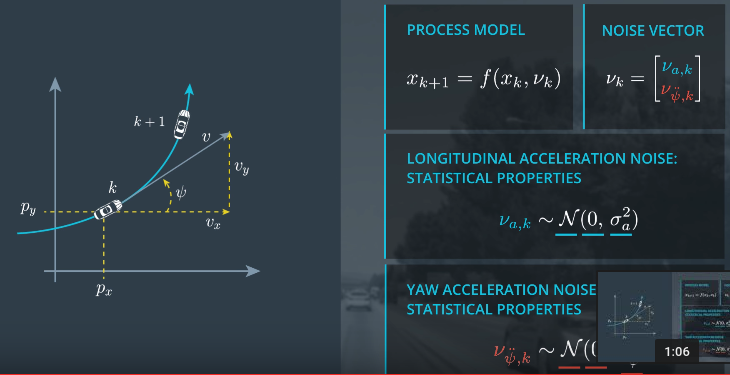
\includegraphics[scale=.5]{4.png}
    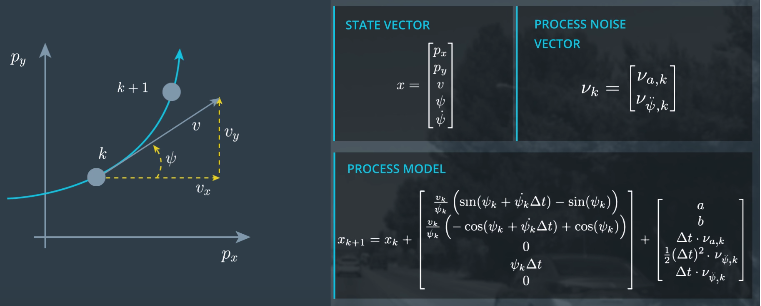
\includegraphics[scale=.5]{5.png}
\end{figure}
\begin{figure}[h!]
  \caption{Sigma point projection from posterior distribution at $k$ to estimate prior state at $k+1$}
  \centering
    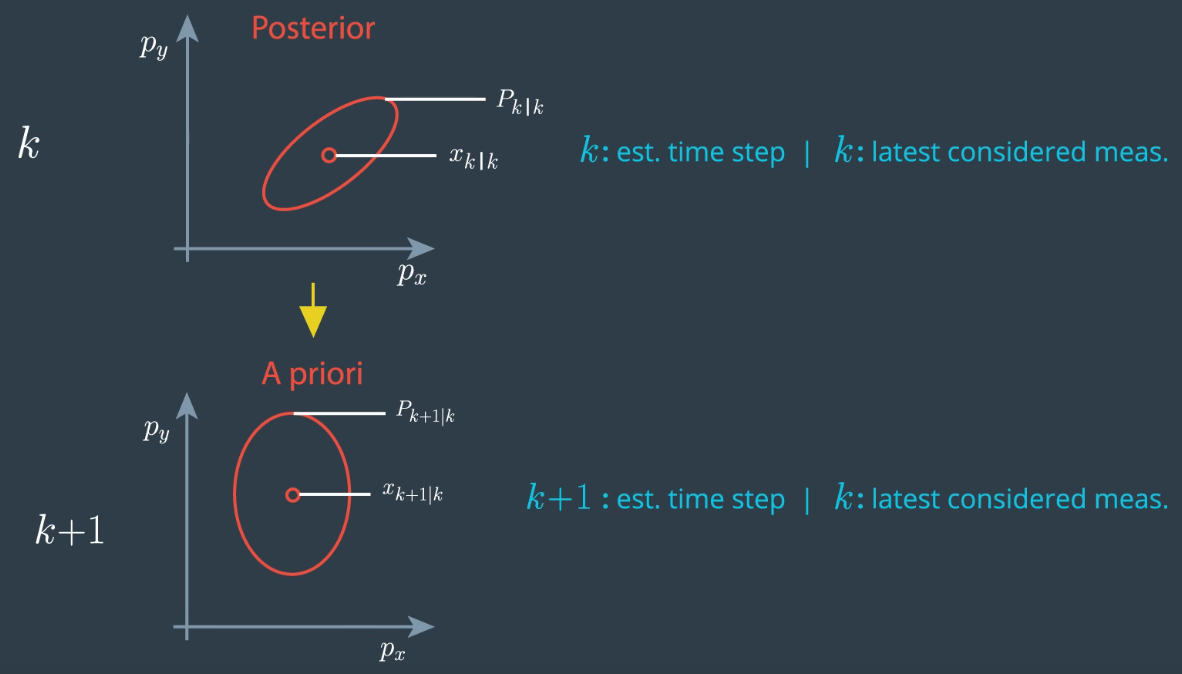
\includegraphics[scale=.15]{6.png}
    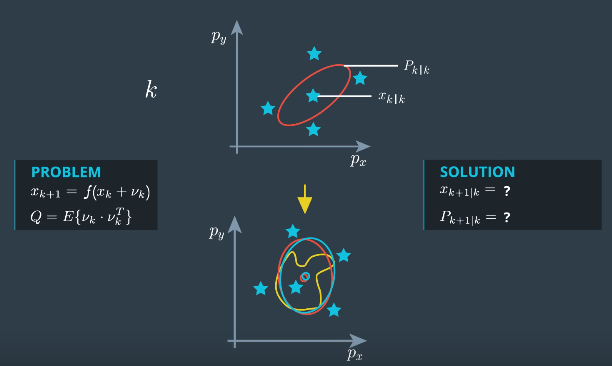
\includegraphics[scale=.3]{7.png}
\end{figure}
\begin{figure}[h!]
  \caption{Details of generating sigma points}
  \centering
    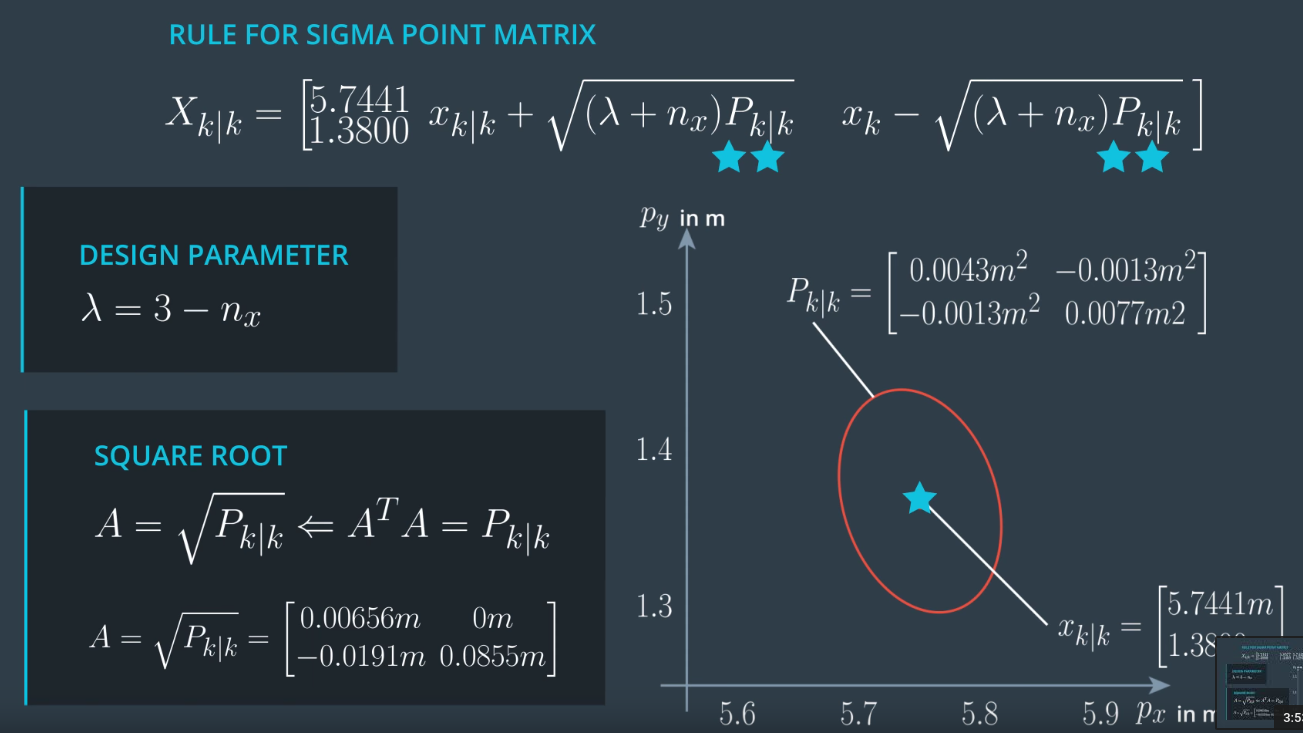
\includegraphics[scale=.15]{8.png}
\end{figure}

\begin{figure}[h!]
  \caption{Augmented sigma points}
  \centering
    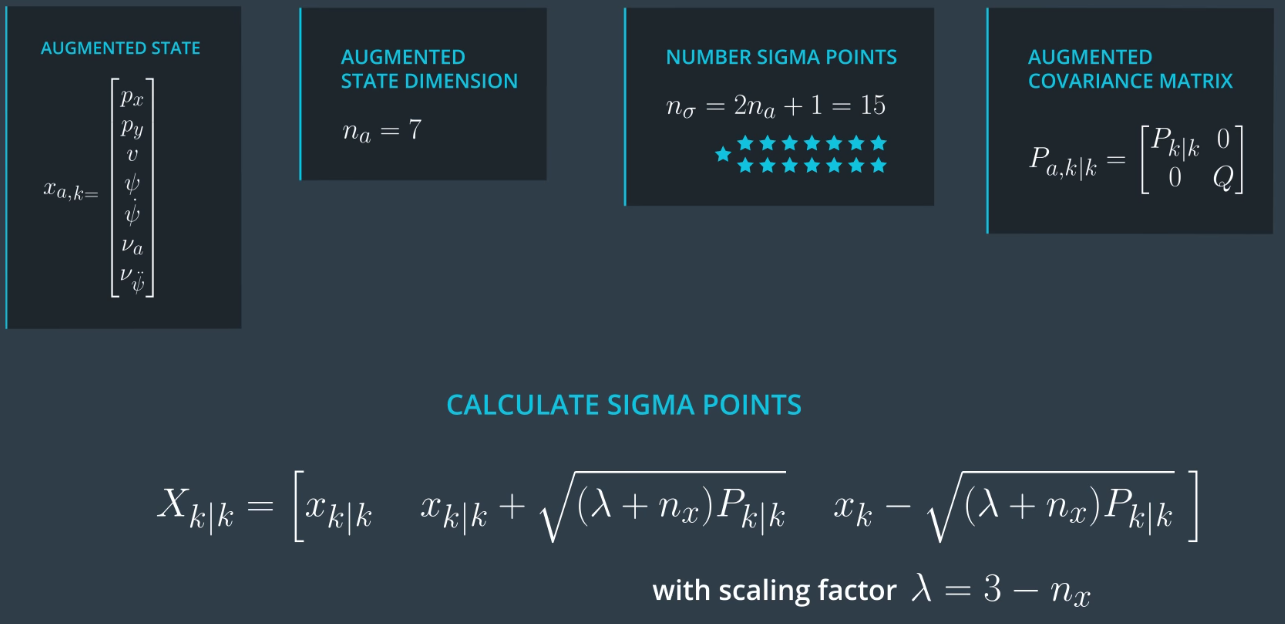
\includegraphics[scale=.15]{9.png}
\end{figure}
\begin{figure}[h!]
  \caption{predicted sigma points throught the process model, and how they are used to estimate the prior distribution of states}
  \centering
    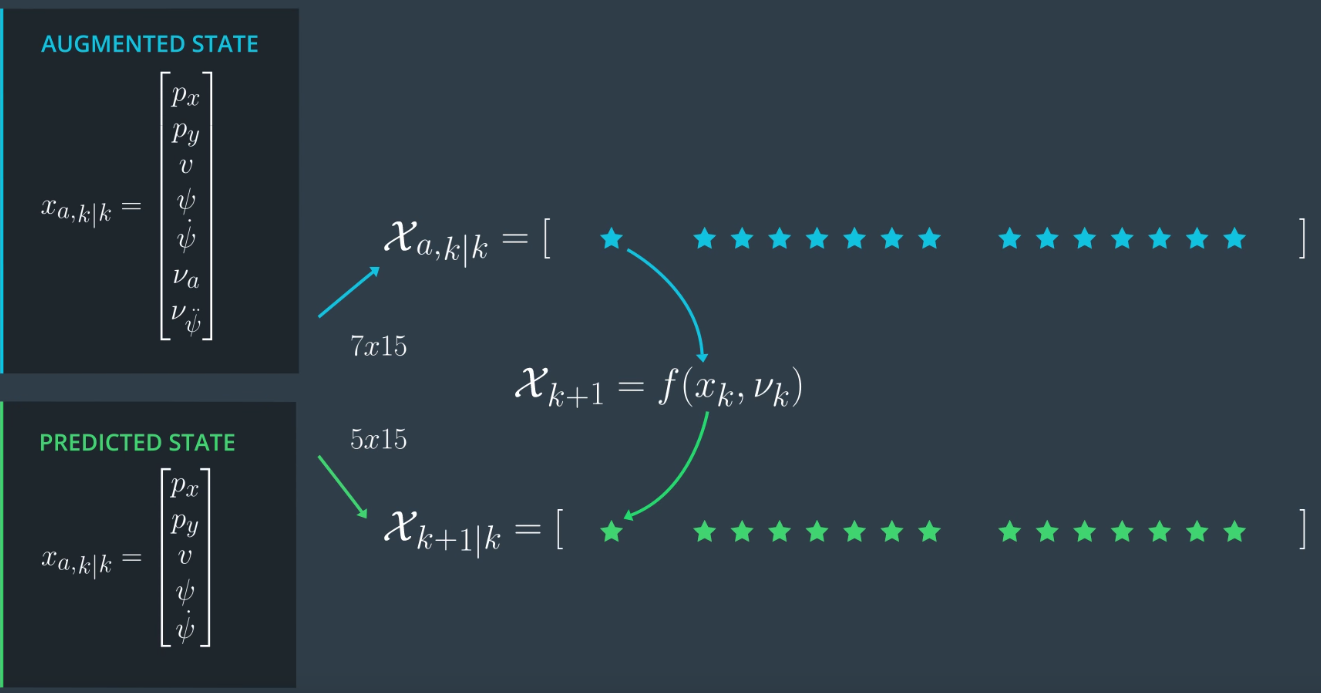
\includegraphics[scale=.15]{10.png}
    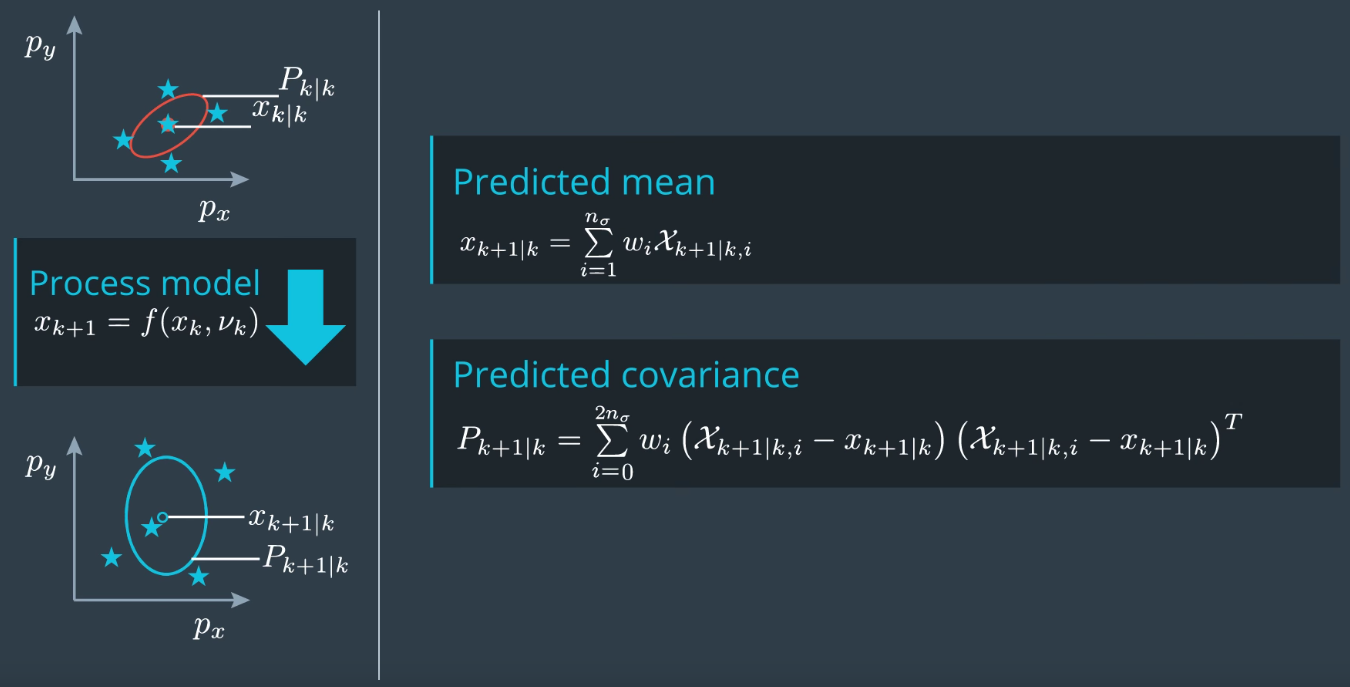
\includegraphics[scale=.15]{11.png}
\end{figure}
\begin{figure}[h!]
  \caption{generating sensor observation sigma points to predict prior distribution of observation before observation is considered at $k+1$}
  \centering
    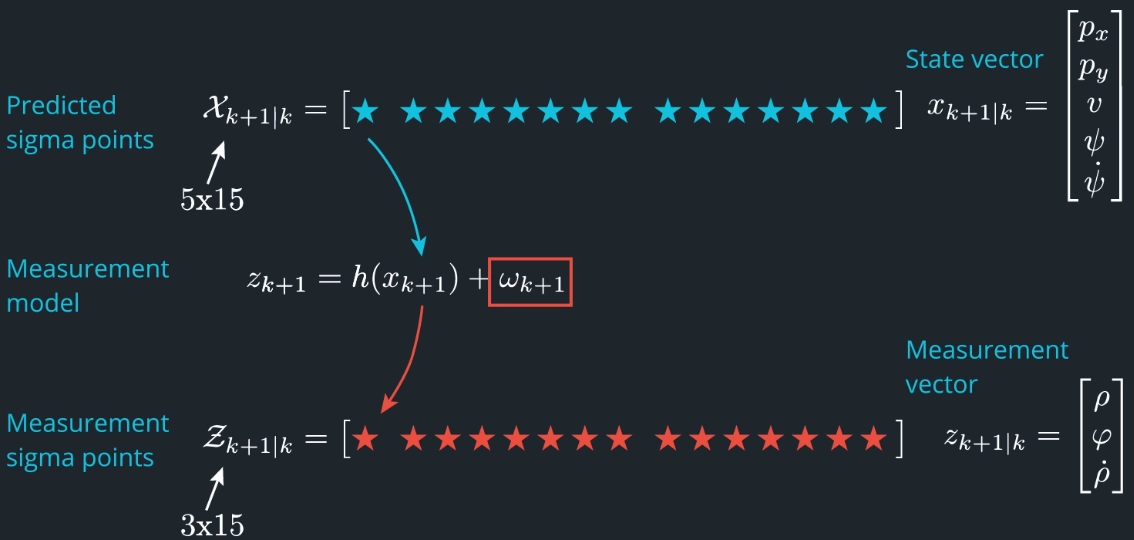
\includegraphics[scale=.2]{12.png}
\end{figure}

\end{document}


